\documentclass{standalone}
\usepackage{pgfplots}
\pgfplotsset{compat=newest}
\usepgfplotslibrary{ternary}
\usepackage{textcomp}
\begin{document}
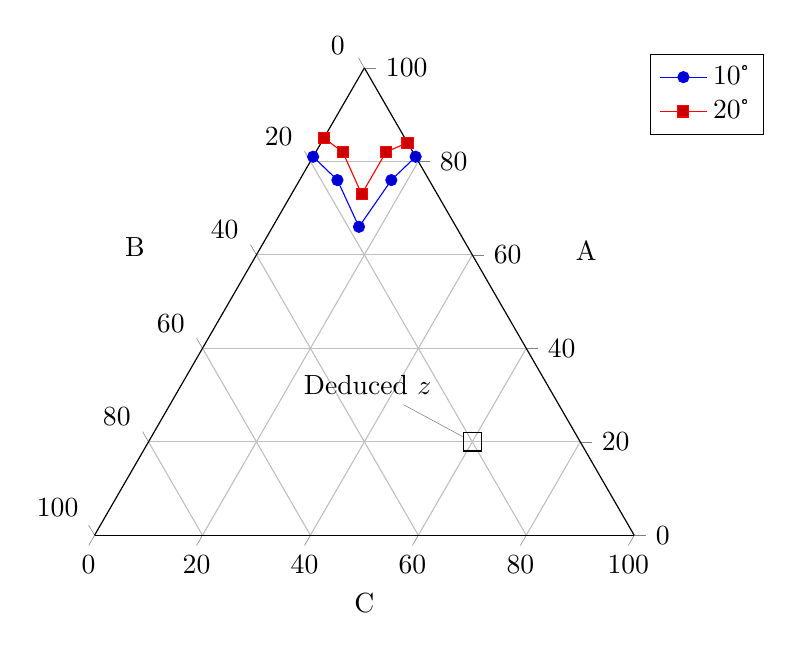
\begin{tikzpicture}
\begin{ternaryaxis}[xlabel=A,ylabel=B,zlabel=C]
	\addplot3 coordinates {
        (0.81,  0.19,  0.00)
        (0.76,  0.17,  0.07)
        (0.66,  0.16,  0.16)
        (0.76,  0.07,  0.17)
        (0.81,  0.00,  0.19)
	};
	\addplot3 coordinates {
        (0.85,  0.15,  0.00)
        (0.82,  0.13,  0.05)
        (0.73,  0.14,  0.13)
        (0.82,  0.06,  0.13)
        (0.84,  0.00,  0.16)
	};
	\node[pin=130:Deduced $z$,draw=black] at (axis cs:0.2,0.2) {};
	\legend{$10$\textdegree, $20$\textdegree}
\end{ternaryaxis}
\end{tikzpicture}
\end{document}
